\section{System Overview}

\begin{outline}
  Present a high-level overview of your proposed control framework,
  likely including a block diagram (similar to Figure 1 in the
  proposal) and a description of each component.
\end{outline}

This work presents a control framework for quadruped robots capable
of generating dynamic, acyclic gaits in challenging environments. The
framework is hierarchical, processing robot state and terrain data to
produce footstep commands for the robot controller.

The first stage of the framework is a footstep evaluation network,
similar to ContactNet from \cite{bratta_contactnet_2024}, which
estimates footstep candidates $\mathbf{f_c}$. The second stage, a
gait generation network (ContactNet), takes these candidates
$\mathbf{f_c}$, ranks them, and outputs the optimal footstep action
$\mathbf{f_a}$ to the robot controller.

This hierarchical design enables strict control over the range of
possible actions the robot can execute. Between the two stages,
candidate actions are filtered to ensure that only valid, prescribed
movements are permitted.

\begin{todo}
  update \autoref{fig:diagram-control-system} with images of my
  environment.   Also update language of different control blocks and
  connections between them.
\end{todo}

\begin{figure}[H]
  \centering
  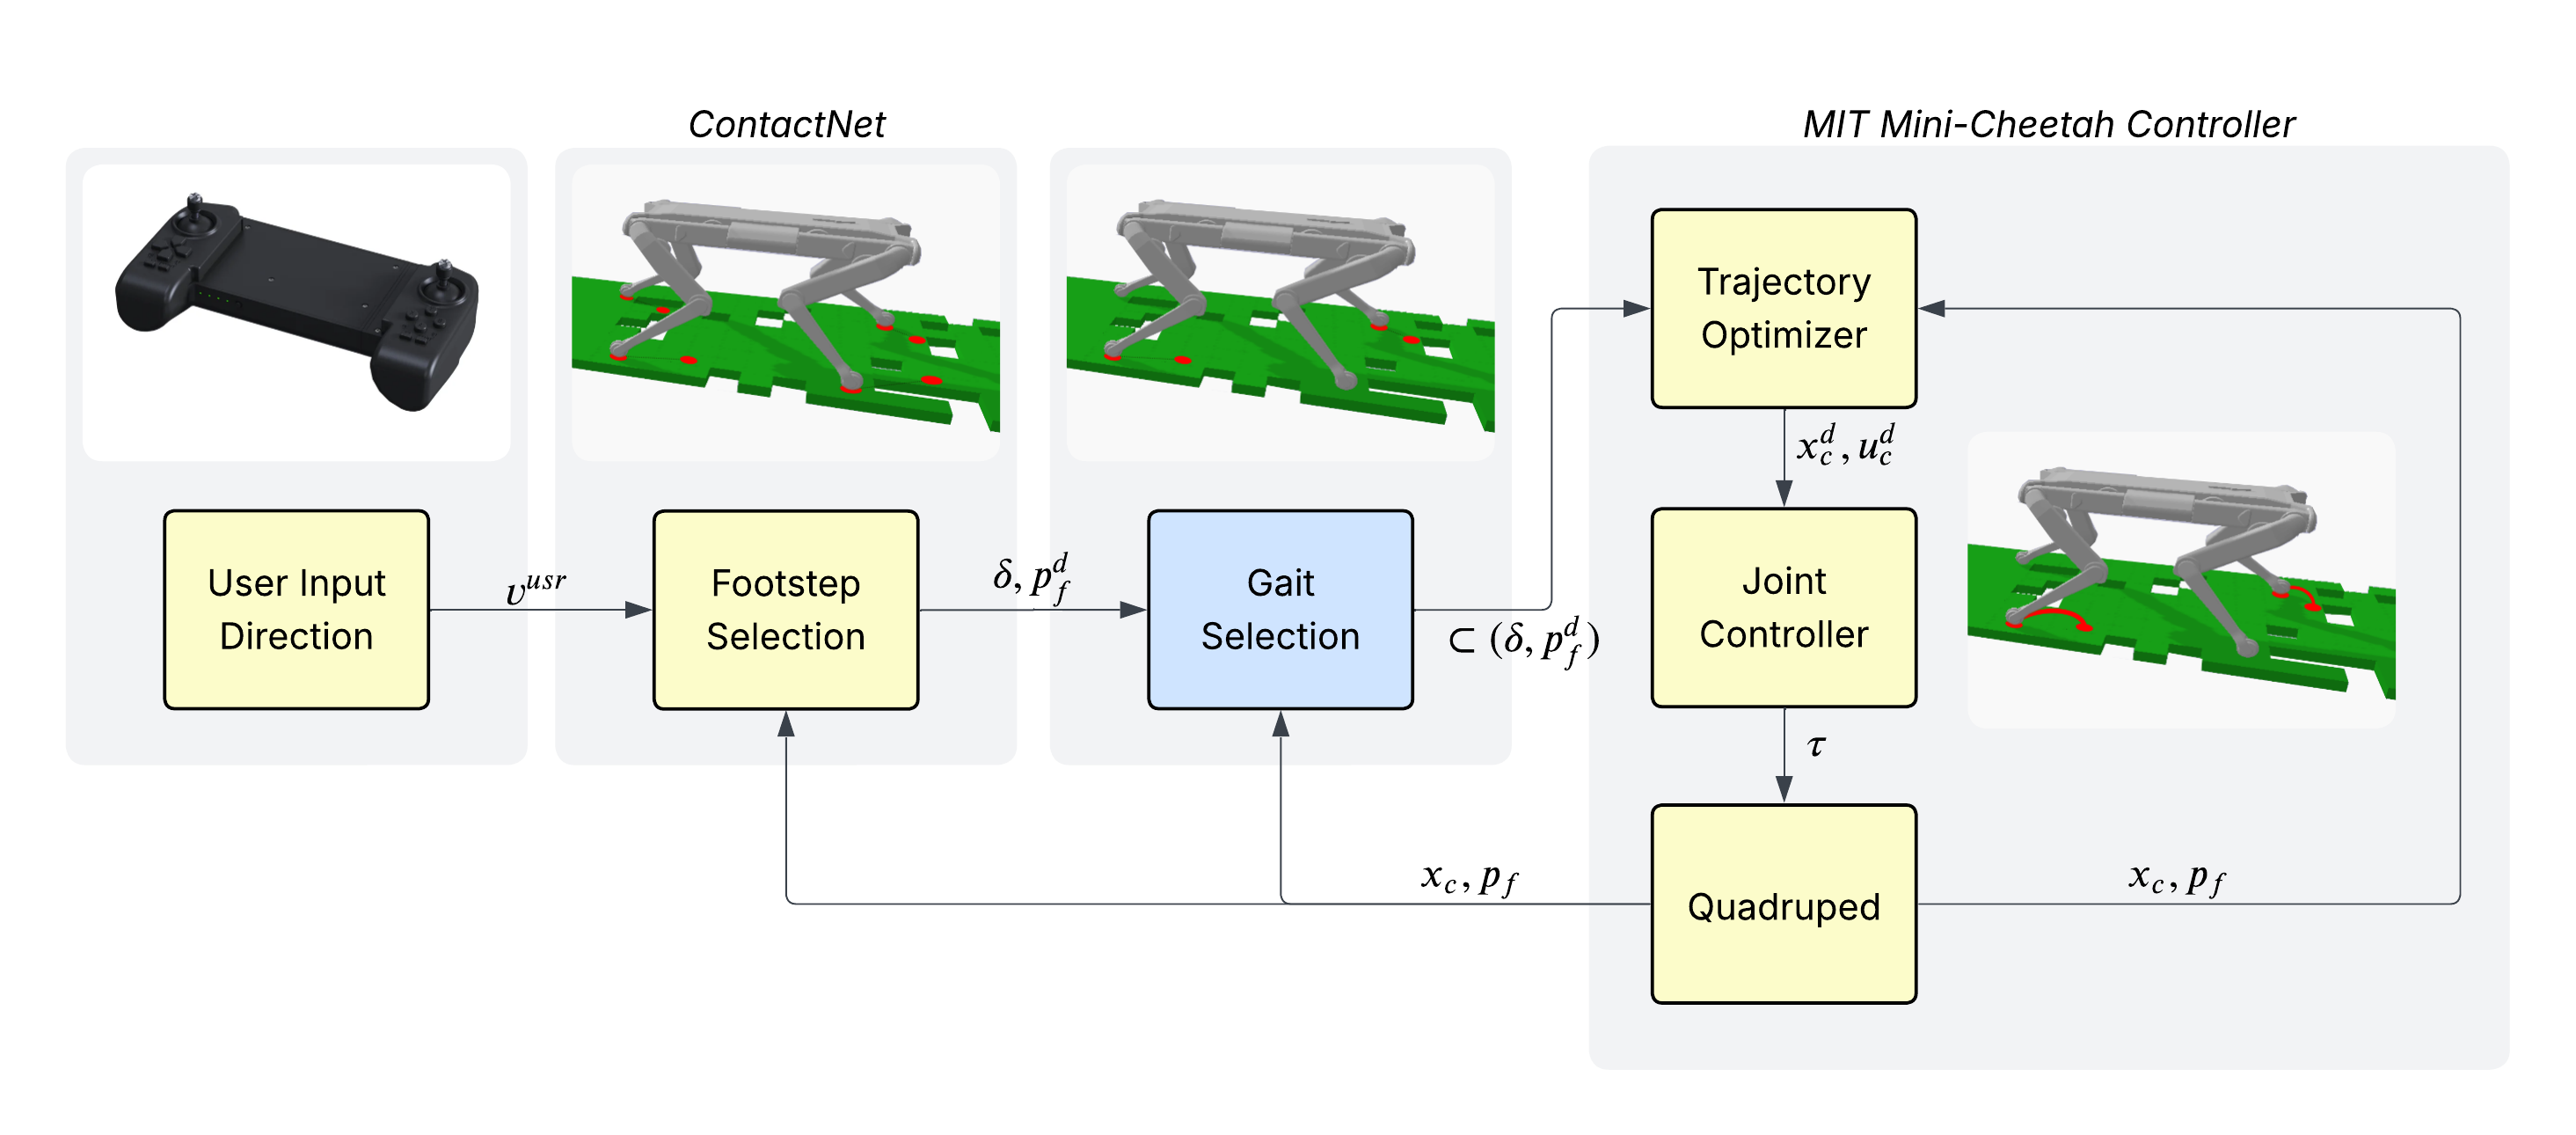
\includegraphics[width=1.0\linewidth]{images/diagrams/control-system.png}
  \caption{A block diagram of the proposed framework. The user
    defines an input direction $v^{usr}$ which the \textit{footstep
    selector} \cite{bratta_contactnet_2024} uses along with, the robot
    state $x_c$, and the current foot positions $p_f$ to generate the
    swing durations $\delta$ and touchdown points $p_f^d$ for all
    currently grounded feet. The \textit{gait selector} (novel) takes
    these desired foot movements and selects an appropriate subset
    $\subset(\delta,p_f^d)$ based on $x_c$, $p_f$, and the terrain
    data. $\subset(\delta,p_f^d)$ is then passed into the MIT
  Mini-Cheetah Controller to perform lower level control.}
  \label{fig:diagram-control-system}
\end{figure}
